\documentclass{package/notes}

%%%%%%%%%% Default Package %%%%%%%%%%%%%
\usepackage{package/color-env}

%%%%%%%%%% Required Packages %%%%%%%%%%%%%
\usepackage{background}
\usepackage[object=vectorian]{pgfornament} %% used in title.tex
\usepackage{braket}
\usepackage{tikz}
\usepackage{subcaption}
\usetikzlibrary{arrows.meta,quantikz}
\usepackage{amssymb,amsmath,amsfonts}  %%% for maths
\usepackage{multicol}
\usepackage{enumitem}
\newlist{gitemize}{itemize}{4}
\setlist[gitemize,1]{
  leftmargin=\dimexpr0.3cm+\labelsep\relax,
  label={\smash{\raisebox{-0.25\height}{
\includegraphics[width=0.6cm]{resources/qc-list-icon.png}}}}
}
\newcommand{\0}{\ket{0}}
\newcommand{\1}{\ket{1}}
%%%%%%%%%%%%%%%%%%%%%%%%%%%%%%%%%%%%%
%%%% Bibliography %%%%%%%%%

\addbibresource{resources/references.bib}
\setcounter{chapter}{-1}
\begin{document}

\begin{titlepage}
\backgroundsetup{contents={}}


\centering % Centre everything on the title page
		
\scshape % Use small caps for all text on the title page

\vspace*{\baselineskip} % White space at the top of the page

%------------------------------------------------
%	Title
%------------------------------------------------

\rule{\textwidth}{1.6pt}\vspace*{-\baselineskip}\vspace*{2pt} % Thick horizontal rule
\rule{\textwidth}{0.4pt} % Thin horizontal rule

\vspace{0.75\baselineskip} % Whitespace above the title
{\huge { Quantum Computing }\\} % Title

\vspace{0.75\baselineskip} % Whitespace below the title

\rule{\textwidth}{0.4pt}\vspace*{-\baselineskip}\vspace{3.2pt} % Thin horizontal rule
\rule{\textwidth}{1.6pt} % Thick horizontal rule

\vspace{2\baselineskip} % Whitespace after the title block

\LARGE{Summer of Science 2021} 

\vspace*{3\baselineskip} % Whitespace under the subtitle



\vspace{0.5\baselineskip} 

{\scshape   \LARGE Eeshaan Jain\\ Mentor: Praveen Sriram} % Editor list

\vspace{0.2\baselineskip} 

\textit{\Large Indian Institute of Technology Bombay} 

\vfill 

\begin{figure}[!h]
    \centering
    
\includegraphics[width=13cm, height=7cm]{resources/quantum-computing-qubit.jpg}
\end{figure}
\vspace{0.3\baselineskip} 


{\large If you can fathom quantum mechanics without getting dizzy, you don't get it. Et kvantebitte spring nærmere supercomputeren\\ - Niels Bohr}
\end{titlepage}

\newpage

\backgroundsetup{contents={}}

\tableofcontents

\chapter{Plan of Action}
\hrule
\vspace{5mm}
\hrule
\vspace{5mm}
\begin{gitemize}
\item \Large{\textbf{Week 0}}
\qquad
Review of Quantum Mechanics
\vspace{5mm}
\hrule
\vspace{5mm}
\item \Large{\textbf{Week 1}}
\qquad
Quantum Circuits
\vspace{5mm}
\hrule
\vspace{5mm}
\item \Large{\textbf{Week 2}}
\qquad
Quantum Fourier transform and Search algorithms
\vspace{5mm}
\hrule
\vspace{5mm}
\item \Large{\textbf{Week 3}}
\qquad
Physical realization of Quantum Computers
\vspace{5mm}
\hrule
\vspace{5mm}
\item \Large{\textbf{Week 4}}
\qquad
NMR
\vspace{5mm}
\hrule
\vspace{5mm}
\item \Large{\textbf{Week 5}}
\qquad
Superconducting Qubits
\vspace{5mm}
\hrule
\vspace{5mm}
\item \Large{\textbf{Week 6}}
\qquad
Spin Qubits
\vspace{5mm}
\hrule
\vspace{5mm}
\item \Large{\textbf{Week 7}}
\qquad
Buffer (to modify PoA as time progresses)
\vspace{5mm}
\hrule
\vspace{5mm}
\hrule
\end{gitemize}
\vspace{5mm}
\colorlet{shadecolor}{orange!12}
\begin{shaded}
\begin{itemize}
\item[$\rhd$] The above schedule is tentative, and bound to change depending on the complexity and nature of the topic going on.
    \item[$\rhd$] The book "Quantum Computation and Quantum Information" by Michael A. Nielsen and Isaac L. Chuang is going to be religiously followed for this SoS. Any other material referenced will be mentioned at the end of the document.
    \item[$\rhd$] The weekly updated notes will be uploaded at
    \begin{itemize}
        \item[$\diamond$] \href{https://github.com/EeshaanJain/Quantum-Computing}{the github repository}
        \item[$\diamond$]
        \href{https://eeshaanjain.github.io/quantum}{my website}
    \end{itemize}
\end{itemize}

\end{shaded}
\newpage

\chapter{Brief Glance at Quantum Computing}
\section{Quantum Bits}
\subsection{Single Qubits}
\begin{definition}[Qubit]{def: qubit}
    A qubit is the mathematical analogue of the classical bit upon which quantum computing and information is based. Unlike a classical bit, the quantum bit can be in $\ket{0}$ state, $\ket{1}$ state, and a state defined by the linear combination i.e 
    \begin{equation} \label{def-qubit}
     \ket{\psi} = \alpha \ket{0} + \beta \ket{1} \qquad \text{where}\quad|\alpha|^2 + |\beta|^2 = 1
     \end{equation}
\end{definition}
Some ways a qubit can be realised are:
\begin{itemize}
\item[$\diamond$] two different polarizations of a photon
\item[$\diamond$] alignment of a nuclear spin in a uniform magnetic field
\item[$\diamond$] two states of an electron orbiting a single atom
\end{itemize}
Since $|\alpha|^2 + |\beta|^2 = 1$, we can write (\ref{def-qubit}) as
\begin{equation}
    \ket{\psi} = e^{\iota\gamma}\bigg(\cos\frac{\theta}{2}\0 + e^{\iota\varphi}\sin\frac{\theta}{2}\1\bigg) \qquad \text{where} \quad \theta, \varphi, \gamma \in \mathbb{R}
\end{equation}
The factor $e^{\iota\gamma}$ doesn't have any observable effect and can be ignored. $\theta$ and $\varphi$ define a point on the unit three-dimensional sphere called the \textit{Bloch sphere} which can be used for visualizing the state of a single qubit (though no simple generalization exists for multiple qubits).
\begin{figure}[h]\label{fig-bloch}
    \centering
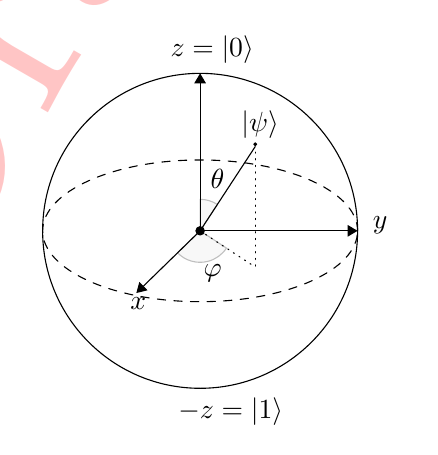
\begin{tikzpicture}[line cap=round, line join=round, >=Triangle]
  \clip(-2.19,-2.49) rectangle (2.66,2.58);
  \draw [shift={(0,0)}, lightgray, fill, fill opacity=0.1] (0,0) -- (56.7:0.4) arc (56.7:90.:0.4) -- cycle;
  \draw [shift={(0,0)}, lightgray, fill, fill opacity=0.1] (0,0) -- (-135.7:0.4) arc (-135.7:-33.2:0.4) -- cycle;
  \draw(0,0) circle (2cm);
  \draw [rotate around={0.:(0.,0.)},dash pattern=on 3pt off 3pt] (0,0) ellipse (2cm and 0.9cm);
  \draw (0,0)-- (0.70,1.07);
  \draw [->] (0,0) -- (0,2);
  \draw [->] (0,0) -- (-0.81,-0.79);
  \draw [->] (0,0) -- (2,0);
  \draw [dotted] (0.7,1)-- (0.7,-0.46);
  \draw [dotted] (0,0)-- (0.7,-0.46);
  \draw (-0.08,-0.3) node[anchor=north west] {$\varphi$};
  \draw (0.01,0.9) node[anchor=north west] {$\theta$};
  \draw (-1.01,-0.72) node[anchor=north west] {$x$};
  \draw (2.07,0.3) node[anchor=north west] {$y$};
  \draw (-0.5,2.6) node[anchor=north west] {$z=\0$};
  \draw (-0.4,-2) node[anchor=north west] {$-z=\1$};
  \draw (0.4,1.65) node[anchor=north west] {$\ket{\psi}$};
  \scriptsize
  \draw [fill] (0,0) circle (1.5pt);
  \draw [fill] (0.7,1.1) circle (0.5pt);
\end{tikzpicture}
\caption{Bloch sphere for a single qubit}
\end{figure}\\
\subsection{Multiple Qubits}
A two qubit system has four computational basis states $\ket{00}\ket{01}\ket{10}\ket{11}$, and the pair can exist in a \textit{superposition} of these too with a complex amplitude as 
\begin{equation}\ket{\psi} = \sum_{i,j \in \{0,1\}} \alpha_{ij}\ket{ij} \qquad\text{where} \quad \sum_{x\in\{0,1\}^2}|\alpha_x|^2 = 1 \end{equation}
It is possible to measure a subset of qubits, say we measure the first qubit alone giving 0 with probability $|\alpha_{00}|^2 + |\alpha_{01}|^2$ leaving the post measurement state as $\ket{\psi'} = \dfrac{\alpha_{00}\ket{00} + \alpha_{01}\ket{01}}{\sqrt{|\alpha_{00}|^2 + |\alpha_{01}|^2}}$. \\
The \textit{Bell states} also called the \textit{EPR pairs} are $\ket{\beta_{xy}} = \dfrac{\ket{0,y} + (-1)^x \ket{1, \bar{y}}}{\sqrt 2}$, i.e
\begin{equation}\label{eq-bell}
    \ket{\beta_{00}} = \dfrac{\ket{00} + \ket{11}}{\sqrt 2}\;,\; \ket{\beta_{01}} = \dfrac{\ket{01} + \ket{10}}{\sqrt 2} \;,\;\ket{\beta_{10}} = \dfrac{\ket{00} - \ket{11}}{\sqrt 2}
    \;,\; \ket{\beta_{11}} = \dfrac{\ket{01} - \ket{10}}{\sqrt 2}
\end{equation}
Upon measuring the first qubit, we can get two results: 
\begin{itemize}
    \item[$\diamond$] 0 with probability $\dfrac{1}{2}$ leaving $\ket{\psi'} = \ket{00}$
    \item[$\diamond$] 1 with probability $\dfrac{1}{2}$ leaving $\ket{\psi'} = \ket{11}$
\end{itemize}
The second qubit always follows the first in terms of measurement, i.e there is correlation between the measurements.
\section{Quantum Computation}
\subsection{Single Qubit Gates}
Let's first define the constraint there exists for a matrix to be called a single qubit gate. Consider the initial state to be $\ket{\psi} = \alpha \ket{0} + \beta \ket{1}$ and the state after the gate has acted to be $\ket{\psi'} = \alpha' \ket{0} + \beta' \ket{1}$. Both of these must satisfy the normalization condition and the matrix $U$ defining the gate must be unitary i.e $$U^\dagger U = I$$
This defines the \textit{only} constraint imposed on quantum gates, and we can clearly see that there exists infinitely many gates. Single qubit gates correspond to rotations and reflections of the Bloch Sphere. \\
Some important gates are: 
\begin{itemize}
    \item[$\diamond$] \textbf{NOT Gate}: The NOT gate takes the state $\alpha \ket{0} + \beta \ket{1}$ to $\alpha \ket{1} + \beta \ket{0}$ and realised as \begin{equation}\label{eq-not}
        X = \begin{bmatrix}
        0 & 1 \\ 1 & 0
        \end{bmatrix}
    \end{equation}
    \item[$\diamond$] \textbf{Z Gate}: Leaves $\0$ unchanged and flips the sign $\1$ and realised as
    \begin{equation}\label{eq-z}
        Z = \begin{bmatrix}
        1& 0 \\ 0 & -1
        \end{bmatrix}
    \end{equation}
    \item[$\diamond$] \textbf{H Gate}: The \textit{Hadamard} gate turns $\0$ to $\dfrac{\0 + \1}{\sqrt 2}$ (first column of $H$) and $\1$ to$\dfrac{\0 - \1}{\sqrt 2}$ (second column of $H$). Note that $H^2 = I$ and thus applying it twice leaves the state unchanged. \\The $H$ operation is a rotation about the $\hat y$ axis by $90^\circ$ followed by about $\hat x$ axis by $180 ^ \circ$
    \begin{equation}\label{eq-h}
        H = \dfrac{1}{\sqrt 2}\begin{bmatrix}
        1& 1 \\ 1 & -1
        \end{bmatrix}
    \end{equation}
\end{itemize}
It can be proven that any arbitrary $2\times2$ unitary matrix can be decomposed as 
\begin{equation}
    U = \underbrace{e^{\iota\alpha}}_{\text{phase shift}}
    \underbrace{
    \begin{bmatrix}
    e^{-\iota\beta / 2} & 0 \\
    0 & e^{\iota\beta / 2}
    \end{bmatrix}}_{\text{rotation about } \hat z\text{ axis}} 
    \underbrace{
    \begin{bmatrix}
    \cos \frac{\gamma}{2} & -\sin\frac{\gamma}{2} \\
    \sin\frac{\gamma}{2} & \cos\frac{\gamma}{2}
    \end{bmatrix}}_{\text{product of rotations}},\quad
    \begin{bmatrix}
    e^{-\iota\delta / 2} & 0 \\
    0 & e^{\iota\delta / 2}
    \end{bmatrix}
\end{equation}
We can build arbitrarily good approximation of gates using special fixed values of $\alpha, \beta$ and $\gamma$. And thus, it is possible to build up an arbitrary single quantum gate using a \textit{finite} set of quantum gates.
\begin{proposition}
AAny arbitrary quantum computation on any number of qubits can be generated by a finite set of gates that is said to be \textit{universal} for quantum computation.
\end{proposition}
\subsection{Multiple Qubit Gates}
A prototypical multi-qubit quantum logic gate is the CNOT (controlled-NOT) gate. The gate takes a control qubit (top) and a target qubit (bottom) and if the control qubit is 0, the target is left alone else it is flipped. The operation is simply $\ket{A, B} \to \ket{A, B\oplus A}$ \\
\vskip.2\baselineskip
\begin{minipage}{0.45\textwidth}
\centering
\begin{quantikz}
\lstick{$\ket{A}$} & \ctrl{1}& \qw\rstick{$\ket{A}$} \\
\lstick{$\ket{B}$} & \targ{}&\qw \rstick{$\ket{B\oplus A}$} \\
\end{quantikz}
\end{minipage}
\begin{minipage}{0.45\textwidth}
\begin{equation}
    U_{CN} = \begin{bmatrix}
    1 & 0 & 0 & 0 \\
    0 & 1 & 0 & 0 \\
    0 & 0 & 0 & 1 \\
    0 & 0 & 1 & 0 
    \end{bmatrix}
\end{equation}
\end{minipage}\\
\vspace{1mm}
The CNOT gate is a type of generalization of the classical XOR gate. But we cannot realize the regular XOR or NAND gate because these operations are \textit{irreversible}, i.e given $A\oplus B$, we cannot get back $A$ and $B$, and an irretrievable loss of information is associated with them. A unitary matrix is always invertible and hence a quantum gate can always be inverted by another quantum gate. 
\begin{theorem}[Universality]{def: universality}
 Any multiple qubit gate may be composed from CNOT and single qubit gates.
\end{theorem}
This is the quantum parallel of the universality of the NAND gate.
\begin{shaded}
\begin{itemize}
    \item[$\diamond$] Given any two basis states $\ket a$ and $\ket b$ for a qubit, it is possible to express an arbitrary state as a linear combination i.e $\alpha \ket{a} + \beta\ket b$ and provided these are orthonormal, we can perform a measurement w.r.t these bases.
\end{itemize}
\end{shaded}
\subsection{Quantum circuits}
A wire in a quantum circuit may not correspond to anything physical. It may be passage of time, or movement of a particle (photon) through space. Conventionally, the state input to the circuit is the computational basis state, i.e all $\0$s.
\subsubsection{The swap operation}
The swap operation swaps the state of the two qubits and can be realised as 
\begin{align*}
    \ket{a,b} &\to \ket{a, a\oplus b} \\
    &\to \ket{a\oplus(a\oplus b), a \oplus b} = \ket{b, a \oplus b} \\
    &\to \ket{b, (a\oplus b)\oplus b} = \ket{b, a}
\end{align*}
\vspace{-2mm}
\begin{figure}[h]
    \centering
    \begin{quantikz}
    &\ctrl{1} &\targ{} & \ctrl{1} & \qw \\
    &\targ{} & \ctrl{-1} & \targ{} & \qw
    \end{quantikz}
    $\qquad\equiv\qquad$
    \begin{quantikz}
    &\swap{1} & \qw \\
    & \targX{}  & \qw
    \end{quantikz}
    \caption{Circuit to swap two qubits}
\end{figure}
\subsubsection{Distinction between classical and quantum circuits}
There are a few things allowed in classical circuits, which aren't in quantum circuits.
\begin{itemize}
    \item[$\diamond$] Loops aren't allowed, hence circuit is acyclic.
    \item[$\diamond$] FanIn and FanOut aren't allowed as these are irreversible, and copying a qubit is forbidden.
\end{itemize}
\begin{shaded}
Just like the CNOT gate, we can make a Controlled-U Gate.
\end{shaded}
\subsubsection{Quantum circuit for teleportation}
\begin{figure}[h]
    \centering
    \begin{quantikz}
    \lstick{$\ket{\psi}$} & \ctrl{1} & \gate{H} & \meter{$M_1$}  & \cw & \cwbend{2}\\
    \lstick[wires=2]{$\ket{\beta_{00}}$} & \targ{} & \qw & \meter{$M_2$} & \cwbend{1} \\
    \qw& \qw & \qw& \qw &\gate{X^{M_2}} & \gate{Z^{M_1}} & \qw \rstick{$\ket{\psi}$}
    \end{quantikz}
    \caption{Quantum circuit for teleporting a qubit}
\end{figure}
\noindent
Consider the state to be teleported as $\ket{\psi} = \alpha\0+\beta\1$ and state input to the circuit is $\ket{\psi_0} = \ket{\psi}\ket{\beta_{00}}$ \\
which is $\dfrac{1}{\sqrt{2}} \Big[\alpha\0(\ket{00}+\ket{11}) + \beta\1(\ket{00}+\ket{11})\Big]$. After passing through the CNOT gate, we get 
\[\ket{\psi_1} = \dfrac{1}{\sqrt 2}\Big[\alpha\0(\ket{00}+\ket{11}) + \beta\1(\ket{01}+\ket{10})\Big]\]
And after passing through the $H$ gate, we get
\begin{align*}
    \ket{\psi_2} &= \dfrac{1}{ 2}\Big[\alpha(\0+\1)(\ket{00}+\ket{11}) + \beta(\0-\1)(\ket{01}+\ket{10})\Big] \\
    &= \dfrac{1}{2}\Big[\ket{00}(\alpha\0+\beta\1)
      + \ket{01}(\alpha\1+\beta\0)+
      \ket{10}(\alpha\0-\beta\1)
      +\ket{11}(\alpha\1-\beta\0)\Big]
\end{align*}
Now after measurement, the receiver should know what the sender has measured to know what gates to apply to get the desired outcome (note that this places the restriction on speed of quantum teleportation). The gates to be applied can be written as $Z^{M_1}X^{M_2}$ where $M_1, M_2 \in \{0,1\}$
\section{Quantum Algorithms}
\subsection{Doing classical computations}
Any classical circuit can be replaced by an equivalent quantum circuit having only reversible elements using the \textit{Toffoli gate}. 
\begin{figure}[h]
    \centering
    \begin{quantikz}
        \lstick{$a$} & \ctrl{1} & \qw\rstick{$a$} \\
        \lstick{$b$} & \ctrl{1} & \qw\rstick{$b$} \\
        \lstick{$c$} & \targ{} & \qw\rstick{$c\oplus ab$}
        \end{quantikz}
    \caption{Toffoli gate circuit \\ If $a,b\neq 1$ then $c$ unchanged else flipped}
\end{figure}\\
Toffoli gate can be used to simulate irreversible classical gates, for example $c=1$ gives us the NAND gate. Putting $a=1$ and $c=0$ gives us a FanOut.
\newpage
\subsection{Quantum Parallelism}
\begin{figure}[h]
    \centering
    \begin{quantikz}
        \lstick{$\dfrac{\0+\1}{\sqrt 2}$}&\gate[wires=2]{U_f}[1.7cm]
            \gateinput{$x$}
            \gateoutput{$x$} &\qw \\
        \lstick{$\0$}& \gateinput{$y$} \gateoutput{$y\oplus f(x)$} &\qw
    \end{quantikz}
    \caption{Circuit demonstrating the formulation below} 
\end{figure}
\noindent
We prepare the data register ($x$) as $\frac{\0+\1}{\sqrt 2}$ (apply $H$ on $\0$) and apply a unitary gate $U_f$ which maps $\ket{x,y} \to \ket{x, y\oplus f(x)}$. This gives us $\frac{\ket{0, f(0)} + \ket{1, f(1)}}{\sqrt 2}$ and we have information about both $f(0)$ and $f(1)$!. Unlike classical circuits, a single $f(x)$ circuit evaluated the values simultaneously. \\
Generalization of the above is called the \textit{Wash-Hadamard transform}. We apply $n$ $H$ gates in parallel to $n$ qubits (denoted as $H^{\otimes n}$), and the result we get is \begin{equation}
    \dfrac{1}{\sqrt{2^n}}\sum_x\ket{x} \quad \text{given that all qubits were initially prepared as }\0
\end{equation}
\subsection{Deutsch's Algorithm}
Modifying the above circuit, 
\begin{figure}[h]
    \centering
    \begin{quantikz}
        \lstick{$\0$}&\gate{H}&\gate[wires=2]{U_f}[1.7cm]
            \gateinput{$x$}
            \gateoutput{$x$} &\gate{H}&\qw \\
        \lstick{$\1$}&\gate{H}& \gateinput{$y$} \gateoutput{$y\oplus f(x)$} &\qw&\qw 
    \end{quantikz}
    \caption{Circuit demonstrating the formulation below} 
\end{figure}\\
\noindent
The input $\ket{\psi_0} = \ket{01}$ and passing through $H$ gives $\ket{\psi_1} = \bigg[\dfrac{\0+\1}{\sqrt 2}\bigg]\bigg[\dfrac{\0-\1}{\sqrt 2}\bigg]$ and noticing that $U_f$ applied to $\ket{x}\dfrac{\0+\1}{\sqrt 2}$ gives $(-1)^{f(x)}\ket{x}\dfrac{\0-\1}{\sqrt 2}$, we can write after applying $U_f$ and taking $H$ on the first qubit,
\[
    \ket{\psi_3} = \begin{cases}
        \pm\0 \dfrac{\0-\1}{\sqrt 2} \qquad \text{if } f(0)=f(1)\\
        \pm\1 \dfrac{\0-\1}{\sqrt 2} \qquad \text{if } f(0) \neq f(1)
    \end{cases}
\]
It can be simplified to
\begin{equation}
    \ket{\psi_3} = \pm \ket{f(0) \oplus f(1)} \bigg[\dfrac{\0-\1}{\sqrt 2}\bigg]
\end{equation}
\subsection{Deustsch-Jozsa Algorithm}
\begin{figure}[h]
    \centering
    \begin{quantikz}
        \lstick{$\0$}&\qwbundle{n}&\gate{H^{\otimes n}}&\gate[wires=2]{U_f}[1.7cm]
            \gateinput{$x$}
            \gateoutput{$x$} &\gate{H^{\otimes n}}&\qw \\
        \lstick{$\1$}&\qw&\gate{H}& \gateinput{$y$} \gateoutput{$y\oplus f(x)$} &\qw&\qw 
    \end{quantikz}
    \caption{Circuit implementing the Deutsch-Josza algorithm} 
\end{figure}
The \textit{Deutsch's problem} is defined as the task to find in the least correspondence if a function $f(x)$ if constant or balanced (equal number of 0 and 1 in output). If the function takes $n$ inputs, classically, we need to query at least $2^n/2 + 1$ times in the worst case. Instead, if we had qubits, we could proceed as follows:
The input state is $\ket{\psi_0} = \0^{\otimes n}\1$ and after passing through the $n+1$ parallel $H$ gates, we get $\ket{\psi_1} = \displaystyle \sum_{x\in\{0,1\}^n}\dfrac{\ket x}{\sqrt{2^n}} \bigg[\dfrac{\0-\1}{\sqrt 2}\bigg]$. Now we apply $U_f$ to get $\ket{\psi_2} = \displaystyle \sum_{x}\dfrac{(-1)^{f(x)}\ket x}{\sqrt{2^n}} \bigg[\dfrac{\0-\1}{\sqrt 2}\bigg]$ \\
Noticing that for a single qubit $H\ket{x} = \sum_z(-1)^{xz}\ket{z}/\sqrt 2$ and expanding for $n$,
\[H^{\otimes n}\ket{x_1, \cdots, x_n} = \dfrac{\sum_{z_1,\cdots,z_n}(-1)^{x_1z_1+\cdots+x_nz_n}\ket{z_1, \cdots, z_n}}{\sqrt{2^n}} = \dfrac{\sum_z (-1)^{x\cdot z}\ket{z}}{\sqrt{2^n}}\]
Thus, 
\begin{equation}
    \ket{\psi_3} = \sum_z\sum_x \dfrac{(-1)^{x\cdot z + f(x)}\ket{z}}{2^n} \bigg[\dfrac{\0-\1}{\sqrt 2}\bigg]
\end{equation}
From this, we measure the query register qubits, and notice that if they are all 0s, we have a constant function else a balanced function.
\subsection{Fourier transform}
We define a linear transformation $U$ on $n$ qubits as 
\begin{equation}
    \ket j \rightarrow \dfrac{1}{\sqrt{2^n}} \sum_{k=0}^{2^n-1} e^{\iota j 2 \pi k / 2^n}\ket k
\end{equation}
Such a transform is unitary, and thus can be realised by a quantum circuit. Moreover, on a superposition :
\begin{equation}
    \sum_{j=0}^{2^n-1}x_j\ket j \to \sum_{k=0}^{2^n-1} \Bigg[\sum_{j=0}^{2^n-1} e^{\iota j 2 \pi k /2^n}x_j\Bigg] \ket k = \sum_{k=0}^{2^n-1}y_k \ket k
\end{equation}
\newpage
\include{2-QM}
 \end{document}
